\documentclass[11pt]{article} % Basic document type
\usepackage{times} % Font 
\usepackage{amsmath} % For matrices
\usepackage{amssymb}
\usepackage[section]{placeins} % Allows FloatBarrier command
\usepackage[utf8]{inputenc} % Font encoding
\usepackage[margin=1.0in]{geometry} % Adjust margins
\usepackage{graphicx} % Allows picture import
\usepackage{pdfpages} % Including pdf files 
\usepackage{setspace}
\usepackage{soul} % Highlighted text
\usepackage{fancyhdr}
\usepackage{appendix}
\usepackage{mcode}
\graphicspath{{images/}} % Allows picture import
\pagestyle{fancy}
\fancyhf{}
\fancyhead[L]{A Real-Time Object Tracking System}
\fancyhead[R]{ECSE 457}
\fancyfoot[C]{\thepage}
\renewcommand{\headrulewidth}{1pt}
\renewcommand{\footrulewidth}{1.5pt}
\newcommand{\HRule}[1][\medskipamount]{\par
  \vspace*{\dimexpr-\parskip-\baselineskip+#1}
  \noindent\rule{\linewidth}{0.2mm}\par
  \vspace*{\dimexpr-\parskip-.5\baselineskip+#1}}
\begin{document}
\begin{titlepage}
\begin{center}
\textsc{\huge McGill University}\\[1.5cm]
\textsc{\LARGE Department of Electrical \& Computer Engineering}\\[1.5cm]
\textsc{\Large ECSE 457 - Final Report}\\[3cm]
\HRule
{\huge \bfseries Research \& Development of a Real-Time Object Tracking System \\[.3cm] }
\HRule 
\vspace{1.5cm}
\noindent
\begin{minipage}{0.4\textwidth}
\begin{flushleft} \large
\emph{\Large Authors:}\\
\vspace{.2cm}
Benjamin \textsc{Brown} \\
\textit{benjamin.brown2@mail.mcgill.ca} \\
260450182 \\
\vspace{.2cm}
Taylor \textsc{Dotsikas} \\
\textit{taylor.dotsikas@mail.mcgill.ca} \\
260457719
\end{flushleft}
\begin{flushleft} \large
\emph{\Large Supervisors:}\\
\vspace{.2cm}
Warren \textsc{Gross, Prof.}\\
\vspace{.2cm}
Arash \textsc{Ardakani} 
\end{flushleft}
\begin{flushleft} \large
\emph{\Large Sponsored by:}\\
\vspace{.2cm}
\textsc{Analog Devices}\\
\end{flushleft}
\end{minipage}%
\end{center}
\end{titlepage}
\pagebreak
\section*{Abstract}
This project aimed to research object tracking algorithms, and implement the algorithm best suited to meet project requirements in both software and hardware. The software implementation used static input videos and the hardware implementation used a real-time input video stream. Phase 1 of the project focused on algorithm research and software implementation, and is documented in \cite{15}. Phase 2 of the project focused on hardware implementation, and this report encompasses all of Phase 2 from the design process to the final results. It was found that hardware implementation of the algorithm provides a much faster way of tracking an object when compared to the equivalent software implementation. It was also found that using a background subtraction, delta frame based algorithm to determine object position is not the best choice for real-time situations, due to the inability to cope with lighting and background variations. It was also found that while a Kalman filter does greatly improve object tracking results, it comes at a heavy cost in terms of hardware utilization.
\section*{Acknowledgments}
We would like to thank Professor Warren Gross and Arash Ardakani for overseeing this project and providing advice, insight, and direction over the course of the year. We would also like to thank Analog Devices for providing us with the Altera DE2 board needed for hardware implementation, and in particular Leah Magaldi for being our main point of contact. Finally, the example TV decoder Verilog code provided by Terasic was a major asset for hardware implementation, we would like to thank them for making it open and available to developers like ourselves. 
\pagebreak
\tableofcontents
\pagebreak
\section{Abbreviations \& Notation}
\begin{itemize}
\item[] FPGA - Field Programmable Gate Array
\item[] VGA - Video Graphics Array
\item[] HDL - Hardware Description Language
\end{itemize}
\section{Introduction}
The ability to determine the position of an object in a scene is a highly relevant challenge for industries like surveillance and robotics. This task represents a challenge from an engineering perspective due to the real-time timing constraints placed on these systems, and the large amount of data that must be processed when working with video data. In order to overcome these challenges, custom hardware implementation has become an increasingly popular solution as demonstrated in \cite{1}, \cite{2}, and \cite{3}. \\\\
\hl{TODO:} This section needs more work.
\section{Background}
This section contains the prerequisite information regarding video tracking needed to understand the system architecture and design. For background information regarding the basics of video processing, Kalman filtering, fixed-point representation, and optical flow, please see \cite{15}. \\\\
\hl{TODO:} Is just referencing this background information enough? Or do we need to repeat the Kalman equations, delta frame generation, and other topics again?
\subsection{Moving Average Filter}
A moving average filter replaces the current input data sample with a mean of some number of past input data samples. The number is referred to as the moving average filter length, $N$. This type of filter is particularly useful when data samples are arriving in a time series (i.e. at constant time intervals) as it will remove outliers, creating a smoother trend in data samples. Given that $p_i$ is the current input data sample, the filtered results, $p_i'$, is given using the following equation,
\begin{equation}
p_i' = \frac{\sum_{k = i}^{i + N} p_{k-N}}{N}
\end{equation}
\subsection{Saturation Filter}
A saturation filter, in the context of this project, refers to either flooring a grayscale pixel intensity to a minimum value or ceiling the grayscale pixel intensity to a maximum value, if it is below or above a threshold. The pseudo-code for the saturation filter is given below.
\begin{lstlisting}
function [output] = saturation_filter(input, min, max, thresh)
	if (input > thresh)
		output = max;
	else
		output = min;
	end
end
\end{lstlisting} 
This makes the data set binary, in the sense that all values are one of two values, and makes data processing significantly easier. In the context of object tracking, values above the threshold indicate an object present in the scene, and values below indicate no object present.
\subsection{Determining Position}
The algorithm implemented in software, and presented in \cite{15}, for determining the $(x,y)$ position of an object in the delta frame used a rastor scan technique to determine the leftmost, rightmost, top, and bottom pixels. By intersecting two lines formed between these points, the center of the object can be estimated. It was found that despite the success of this algorithm in software, it would not be conducive to hardware implementation. This is mainly due to the fact that in the software implementation, data arrived in discrete frames from MATLAB's \texttt{VideoReader} class at constant time steps. In hardware implementation, data is handled at the pixel level, with a constant stream of pixels being placed in and extracted from a FIFO frame buffer storage module (to be discussed later). Thus using an algorithm that requires an entire frame requires more memory and extra logic. A new algorithm was developed to determine the local of the object. \\\\
This algorithm assumes that pixel data arrives in binary format; either a string of all zeros representing no object present or a string of all ones representing an object present. Note that this data format is achieved by using the saturation filter just discussed. The algorithm tests if the pixel is an object pixel or not, and if it is the $x$ and $y$ coordinates of the pixel are each added to a rolling summation ($x_{sum}$ and $y_{sum}$). A counter, $n$, is also incremented At the end of the frame, the rolling summations are divided by the counter, the position is outputted, and the three values are cleared. This algorithm is essentially just taking an average of the $(x,y)$ coordinates of the object pixels as the center of the object.
\begin{equation}
x = \frac{x_{sum}}{n}
\end{equation} 
\begin{equation}
y = \frac{y_{sum}}{n}
\end{equation} 
Note that this algorithm achieves best results when the object is highly symmetric.
\subsection{Video Pipeline}
The phrase \textit{video pipeline} refers to a series of image processing modules that exist between the video input device (e.g. the camera) and the video output device (e.g. the display). The pipeline can be implemented in software or hardware, but for the scope of this report the pipeline will refer to hardware implementation, and modules will be referred to in the Verilog sense. Modules in the video pipeline generally consist of decoding and encoding the video data into various formats, and performing video processing (e.g. applying algorithms of interest) in the middle. Implementing a video pipeline is directly coupled with implementing an object tracking algorithm in hardware, as there are no libraries or classes to convert and store the incoming video data when working at this low of a level.
\subsection{The VGA Interface}
The ADV7123 High-Speed Video DAC converts three 10-bit RGB digital signals to the corresponding analog signals needed to transmit video data using the VGA interface. To give the user flexibility with timing and resolution, it does not generate the digital synchronization signals. These two signals are horizontal and vertical synchronization (sync). To properly generate these signals and thus drive the VGA interface, the VGA timing specifications must be understood. \\\\ 
A VGA display generates images using a rastor scan technique. The display is a grid of pixels, and each pixel is displayed individually starting at the top left corner, moving left to right in rows, and ending in the bottom right corner. This operation occurs at a speed known as the refresh rate. The refresh rate is fast enough such that the user perceives an entire image display instantaneously, despite the fact that the image is being displayed discretely per pixel. Due to the motion just described, VGA timing specifications are described in terms of horizontal (i.e. the rows) and vertical (i.e. the number of rows) parameters. VGA resolution is described in terms of the number of visible pixels in a single row, and the total number of visible rows in the display. It is important to note that the number of visible pixels and rows is less than the total number of pixels and rows, as there are blanking periods due to timing constraints. The final term that should be defined is the pixel clock, $f_{pixel}$. The pixel clock is used to count each pixel in the grid, and is much faster than the refresh rate. In fact, the refresh rate of a VGA display can be related to the pixel clock and VGA resolution,
\begin{equation}
f_{refresh} = \frac{f_{pixel}}{H_{pixels} \times V_{lines}}
\end{equation}
 Figure \ref{fig:vgaTiming} shows the timing specifications, and has four notable regions: front porch, back porch, sync, and active video \cite{16}. 
\begin{figure}[h]
\centering
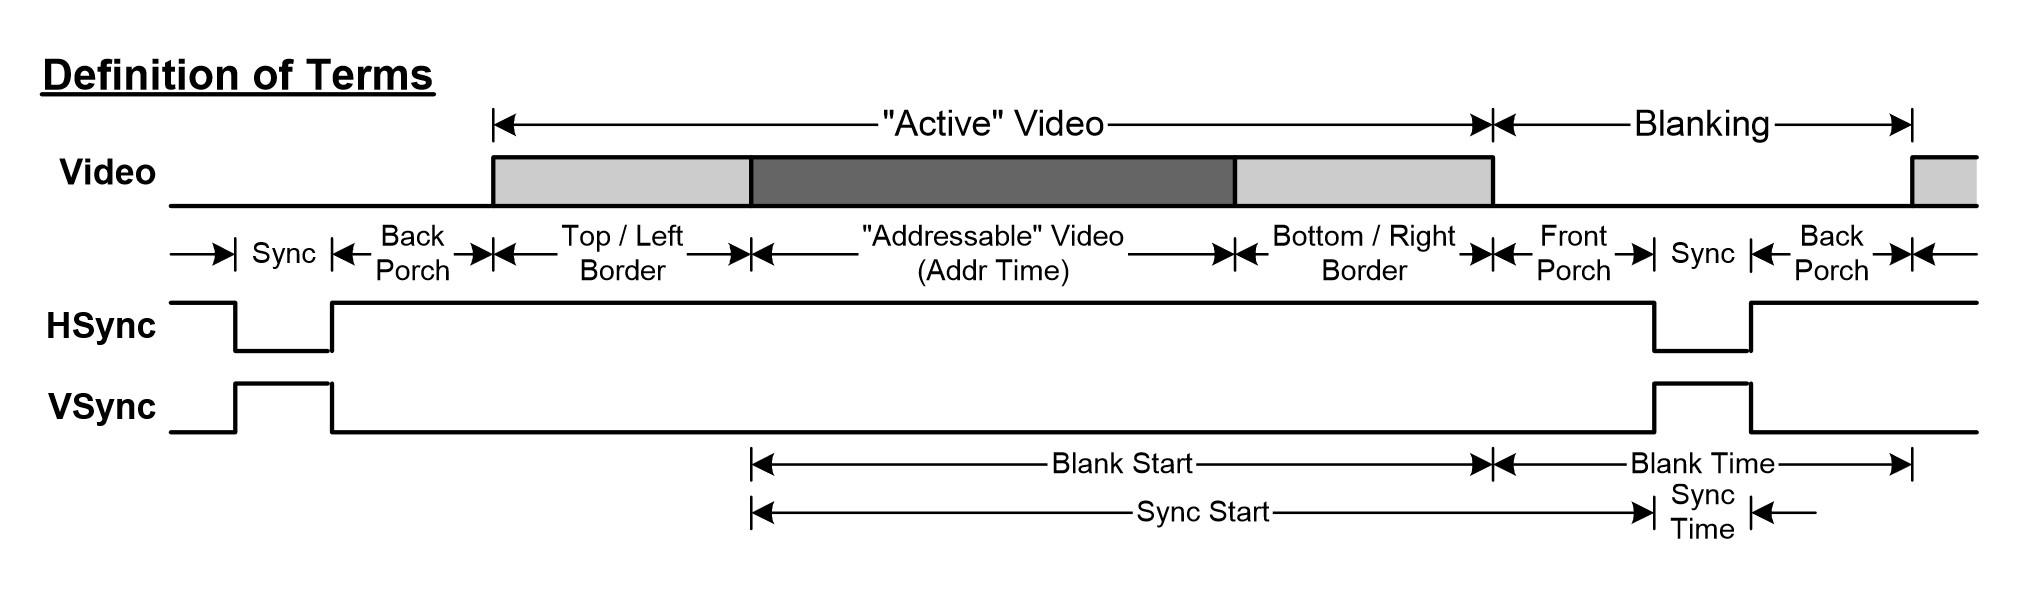
\includegraphics[width=0.8\textwidth]{./images/vgaTiming.jpg}
\caption{VGA Timing Signals \cite{16}}
\label{fig:vgaTiming}
\end{figure}
As the figure shows, the front porch, back porch, and sync regions form what is known as the blanking period, since no valid video data is displayed during this period. The horizontal sync signal must be pulsed (high or low depending on polarity) prior to the valid data is displayed on each row, for a specific amount of time depending on resolution. Similarly, the vertical sync signal must be pulsed prior to the entire frame is displayed. For the typical $640 \times 480$ VGA resolution, the timing constraints shown in Table \ref{table:vga}. \\\\
\begin{table}[h]
\centering
\caption{$640 \times 480$ VGA Timing Specifications \cite{16}}
\label{table:vga}
 \begin{tabular}{ | p{4cm} | p{4cm} | p{4cm} |} \hline
Region & Time & Pixels \\ \hline
Hor. Front Porch & .636 us & 16 \\ \hline
Hor. Sync Period & 3.813 us & 96\\ \hline
Hor. Back Porch & 1.906 us & 48\\ \hline
Hor. Visible & 25.422 us & 640\\ \hline
Ver. Front Porch & 0.317 ms & 10 \\ \hline
Ver. Sync Period & 0.064 ms & 2 \\ \hline
Ver. Back Porch & 1.048 ms & 33 \\ \hline
Ver. Visible & 15.523 ms & 480\\ \hline
\end{tabular}
\end{table}
\textit{Note: Some specifications, such as \cite{16}, add two more regions denoted left and right borders. However, since they are functionally irrelevant for this application, they have been lumped into the front and back porches respectively for this discussion.}
\section{Requirements}
Due to the fact that the scope of the project did not change between Phases 1 and 2, the requirements listed in this section are largely based off of the Phase 1 report \cite{15}. Some additional requirements were added at the beginning of Phase 2 when hardware implementation became clearer.
\subsection{Time Frame}
The project shall be completed by December 2015. The project will be broken into two phases. Phase 1 of the project will be January - April 2015, and Phase 2 of the project will be September - December 2015.
\subsection{Algorithm}
An algorithm shall be chosen such that the system is capable of tracking an object that is in motion, in real-time. The algorithm will be simple enough such that it can be implemented in hardware within the project's duration and within the scope of the author's skills. To ensure this, the chosen algorithm will contain basic operations in order to ease hardware implementation. The algorithm will be chosen during Phase 1 of the project.
\subsection{Software}
Software implementation of the algorithm shall be performed during Phase 1 of the project to act as a proof of concept for the algorithm, and to understand the strengths and weaknesses of the algorithm. Software implementation shall be performed in MATLAB. Upon completion, the software will be able to track an object in motion with a clear and visible cursor, for an input video that satisfies all assumptions and prerequisite conditions the algorithm may have. 
\subsubsection{Floating-Point}
The first iteration of the software implementation shall be in floating-point to provide a high-level structure of the algorithm. The software shall not have any dependencies on MATLAB (i.e. use built in functions) with the exception of simple helper functions such as \texttt{eye}, \texttt{zeros}, \texttt{round}, and \texttt{fix}. MATLAB's \texttt{VideoReader} and \texttt{VideoWriter} class may be used for I/O.
\subsubsection{Fixed-Point}
The second iteration of the software implementation shall be in fixed-point to make hardware implementation easier and more efficient. No values in the fixed-point software shall have fractional portions (e.g. reals, floats, or doubles) with the exception of constants declared directly before conversion and preparing data for MATLAB's \texttt{VideoWriter} class as output.
\subsection{Hardware}
Hardware implementation of the algorithm shall be performed during Phase 2 of the project. The completed hardware implementation of the algorithm shall be the final system. The system will contain embedded hardware which the algorithm has been implemented on. The system will include a video camera providing a live feed of the chosen scene. Upon completion, the system will be able to track an object in motion in real-time and identify the object in motion on a display with a clear and visible cursor. All components of the system shall be as low priced as possible.
\subsubsection{Platform}
The system hardware shall be an Altera DE2 breakout board. This breakout board contains video input/output peripherals, off-chip memory, and an FPGA (Altera Cyclone IV) that contains more than enough resources for the system.
\subsubsection{Method}
The system hardware shall be implemented using Verilog HDL. The sample designs included with the Altera DE2 breakout board include Verilog modules for video input decoding. In order to utilize these resources and avoid mixing languages, Verilog is the logical choice.
\section{Design}
\subsection{Generating VGA Output}
Make sure mention the design references for this.
\subsection{Simple Video Pipeline}
This is where you should cite \cite{13} and talk about the video input wrapper module.
\subsection{Storing the Base Frame}
This is where you should cite \cite{14} and talk about the SRAM.
\subsection{RGB to Grayscale Conversion}
The purpose of this module is to convert RGB values into a single grayscale value. The sample video pipeline provided by Terasic (encapsulated into the "Video Input" module) outputs red, green, and blue pixel data into separate 10-bit registers. For simplicity in thresholding, filtering, and subsequent delta frame generation, it was not necessary to handle 3 channels of data. Converting to a single grayscale value would be sufficient for the rest of the algorithm's implementation. A grayscale value, or luminance $Y$, is achieved by performing a weighted sum of the RGB values,
\begin{equation}
Y =  0.2126\times R + 0.7152\times G + 0.0722\times B
\end{equation}
The coefficients represent the measured intensity perception of typical human eyesight. The resulting grayscale value will be in the range from 0 (total black) to 255 (total white). This equation had to be adjusted for fixed point arithmetic since it uses fractional coefficients. A fractional width of 6 was used. The coefficients were converted to binary and left shifted by 6. The output grayscale value only maintains the most significant 10 bits of the calculation, essentially slicing the fractional portion to obtain the correct result. The equation is performed when a valid data signal is enabled by the previous "Video Input" module. A valid out signal was also introduced to maintain synchronization for the next module in the pipeline. This signal is enabled when valid input data is ready. 

\subsection{Modified Video Pipeline}
Talk about moving the RGB conversion further upstream prior to the SDRAM such that we can work in RGB.
\subsubsection{Delta Frame Generation}
Discuss the poor man's absolute value implemented and the saturation filter.
\subsubsection{Moving Average Filter}
Show the two pictures of the before/after moving average filter here.
\subsection{Measuring Object Position}
The delta frame data is used to identify the $(x,y)$ coordinates of the object. For this step in the pipeline, one module was designed to calculate the $(x,y)$ coordinate, marking the centre of the object in the frame. Another module was developed to colour the location of the object in the frame for visual identification on the monitor. \\\\
To measure the position of the object, several input data sources were utilized. The input delta frame data is binary. All ones in the delta frame register represent and object pixel, while all zeroes represents the background. When an object pixel is received, the register that holds the total number of object pixels is incremented and the $x$ and $y$ coordinate sum registers are also respectively incremented by the current $x$ and $y$ locations of the object pixel in the frame. The $x$ and $y$ locations are received from the VGA module position outputs. These position sources were used instead of internal counters to ensure that processing is synchronized with the output. Using this process, all the necessary data for equations (2) and (3) are satisfied and the calculation can be preformed under a valid signal condition to obtain the centre of the object. The result is calculated and ready for output when the last pixel in the frame is received and processed. At the beginning of each new frame all data is reset for a fresh calculation. The end of the frame is identified when the $x$ and $y$ location values have reached their max resolution values of 640 and 480 respectively. If no object is in the frame, we don't want to identify noise as an object. To prevent this from happening, a simple threshold was implemented. If the total count of object pixels is less than 40 then the $x$ and $y$ location will be set to a value that is not to be displayed on the monitor. \\\\
The second module utilizes the raw $(x,y)$ coordinates and the updated Kalman $(x,y)$ coordinates to display visual identification of the object on the monitor. The pixels around the raw coordinates are coloured as a red box while the pixels around the Kalman coordinates are coloured as a green box. The incoming $(x,y)$ VGA position coordinate is monitored. If a $(x,y)$ position is within 20 pixels of the object's position, then that pixel is coloured red. The same process is repeated comparing VGA position to Kalman $(x,y)$ coordinates, but instead colouring the pixels green. The result on the monitor shows a red box tracking the object and a green box following the object moving accordingly to Kalman filter specifications. 

\subsection{Kalman Filter}
Lots of meat here.
\section{Testing \& Verification}
\hl{TODO:} This section.
\section{Impact on Society}
Since the scope and application of the project did not change between Phases 1 and 2, discussion of the project's impact on society is entirely based off of the Phase 1 report \cite{15}. \\\\
Our dedicated hardware object tracking system will have some impacts in society, but no profound negative impacts. The most notable impact will be its automating effect in the applications it is integrated with. Its introduction to another system will fulfill a task that could have been previously accomplished by a human or even by software previously embedded within the system. The consumer would have to purchase our hardware to implement our system. Our choice of hardware, the Altera DE2 Board has an upfront cost of around \textdollar500. This can be a substantial price for the consumer but the performance benefits outweigh that of embedded software, and in the case of surveillance for example, the cost of running our system will be less than paying a worker to watch a video feed for objects. The introduction of new technology that makes a manned job obsolete is often viewed as a negative impact on society, but this sort of progress is inevitable. \\\\
In the design process so far, we have not made any sort of environmental impact as we have just been developing software. Our system is going to be a combination of previously manufactured parts which were presumably made with the environment in mind. There are so many electronics already in use in society today, the addition of our system's environmental impact can not be quantified. Our product does not produce waste nor does it need constant physical additions. It requires a small constant supply of electricity. When it is no longer needed it can be properly recycled in the same way that computers and other electronics are. Our system does not pose any health or safety risks.\\\\
As mentioned earlier, the value of our device comes from the additional performance gained by a secondary system using it. It is possible that the secondary system has some sort of malicious intent but our product cannot be responsible for any negative consequences the secondary system produces. 
\section{Allocation of Work}
\section{Conclusion}
The final hardware implementation was a success, and the system can display a red dot that shows the $(x,y)$ measurement of the object in the frame as well as green dot showing the improved $(x',y')$ position the Kalman filter produces. Due to the underlying principles of the delta frame generation, the system is an object tracking algorithm and not a motion tracking algorithm. However, the Kalman filter theoretical model assumes constant velocity.This is why when the object stops moving, the green dot slowly converges to the red one. This shows the system favoring the measurements over the model to reduce error, and demonstrates the Kalman filter functioning properly. When the object is moving with constant velocity, the Kalman filter provides a smoother, improved output.
\subsection{Future Work}
\subsubsection{Underlying Algorithm}
The system could be significantly improved by using an object measurement algorithm that has fewer requirements and assumptions regarding the environment. To produce a valid delta frame, the scene background must have constant lighting and no objects in it. In a real-time situation, we found it very difficult to ensure these requirements were met. 
\subsubsection{Motion Tracking}
The delta frame generation algorithm detects objects in the scene regardless of whether or not they are in motion. However the Kalman filter assume a constant velocity model, which means that when it receives measurements they might break this model. In order to ensure the scene reflects the model, the underlying algorithm just mentioned could be modified to be a motion tracking algorithm instead of an object tracking algorithm. We have discussed and attempted to implement this by simply constantly grabbing a new base frame. The idea is that if the base frame is updated very frequently, only objects in motion will be measured.
\subsubsection{Feature or Color Detection}
Using specific color or feature detection could be a major system improvement, and would be more useful for applications like surveillance. The simple averaging algorithm implemented for object measurement assumes highly symmetric objects and is perhaps the simplest possible way of locating an object in a scene. This improvement would require more complicated video processing, and using color would require major changes to the system architecture, which was designed for grayscale.
\newpage
\begin{thebibliography}{11}
\bibitem{1}
F. Roth, “Using low cost FPGAs for realtime video processing”, M.S. thesis, Faculty of Informatics, Masaryk University, 2011.
\bibitem{2}
A. Saeed et al., “FPGA based Real-time Target Tracking on a Mobile Platform,” in 2010 International Conference on Computational Intelligence and Communication Networks, 2010, pp. 560-564.
\bibitem{3}
”Video and Image Processing Design Using FPGAs.” Altera. 2007. January 2014. 
http://www.altera.com/literature/wp/wp-video0306.pdf  
\bibitem{4}
E. Trucco and A. Verri, “Chapter 8 - Motion,” in Introductory Techniques for 3D Computer, pp. 177- 219.
\bibitem{5}
S.A. El-Azim et al., “An Efficient Object Tracking Technique Using Block-Matching Algorithm”, in Nineteenth National Radio Science Conference, Alexandria, 2002, pp. 427 - 433.
\bibitem{6} 
Caner et al., “An Adaptive Filtering Framework For Image Registration”, IEEE Trans. Acoustics, Speech, and Signal Processing, vol. 2, no. 2, 885-888. March, 2005. 
\bibitem{7}
Yin et al. \textit{Performance Evaluation of Object Tracking Algorithm} [Online]. Available: http://dircweb.kingston.ac.uk/ 
\bibitem{8}
G. Shrikanth, K. Subramanian, “Implementation of FPGA-Based object tracking algorithm,” Electronics and Communication Engineering Sri Venkateswara College of Engineering, 2008.
\bibitem{9}
E. Pizzini, D. Thomas, “FPGA Based Kalman Filter,” Worcester Polytechnic Institute, 2012.
\bibitem{10}
M. Shabany. (2011, December 27). \textit{Floating-point to Fixed-point Conversion} [Online]. Available: http://ee.sharif.edu/~digitalvlsi/Docs/Fixed-Point.pdf
\bibitem{11} 
N. Devillard. (1998, July). \textit{Fast median search: an ANSI C implementation} [Online]. Available: http://ndevilla.free.fr/median/median.pdf
\bibitem{12}
D. Kohanbash. (2014, January 30). \textit{Kalman Filtering - A Practical Implementation Guide (with code!)} [Online]. Available: http://robotsforroboticists.com/kalman-filtering/
\bibitem{13} Recommendation ITU-R BT.656-5 (12/2007). “Interface for digital component video signals in 525-line and 625-line television systems operating at the 4:2:2 level of Recommendation ITU-R BT.601". 
\bibitem{14} ISSI Datasheet: “1M x 16 High-Speed Asynchronous CMOS Static RAM with 3.3V Supply".
\bibitem{15} B. Brown \& T. Dotsikas, “A Real-Time Object Tracking System”, ECSE 456 Final Report, unpublished.
\bibitem{16} \textit{VESA and Industry Standards and Guidelines for Computer Display Monitor Timing (DMT)}, Video Electronics Standards Association, Version 1, Revision 11.
\end{thebibliography}
\newpage
\appendix
\appendixpage
\end{document}